\documentclass[pdf, hyperref={unicode}, aspectratio=169]{beamer}

\usepackage{./diploma-slides-latex-template/styles}

% Включаю кнопочки
\setbeamertemplate{navigation symbols}[default]

% Название темы слишком длинное, поменьше шрифт!
\setbeamerfont{title}{series=\bfseries, size=\large}
\setbeamerfont{footline}{series=\bfseries, size=\fontsize{5}{3}\selectfont}

\useoutertheme{miniframes}

\title{Проектирование системы переноса и генерации взаимосвязанных данных из производственной среды при тестировании образовательной платформы}

\subtitle{Выпускная квалификационная работа бакалавра}

\pdfstringdefDisableCommands{
\def\\{}
\def\,{}
\def\textbf#1{<#1>}
}

\author[Мезенин Олег Александрович]
{
	\textbf{Студент группы М8О-406Б-21:} Мезенин Олег Александрович\\
	\ \textbf{Научный руководитель:} ст. преподаватель кафедры 806\\\ Миронов Евгений Сергеевич
	% Обратите внимание на пробел в начале строки
}

\institute[Московский авиационный институт]
{
	Московский авиационный институт (национальный исследовательский университет)\\
	Институт № 8 «Компьютерные науки и прикладная математика»\\
	Кафедра № 806 «Вычислительная математика и программирование» 
}

\date{Москва --- \the\year}

\logo{
\includegraphics[height=1cm]{img/mai}}


\begin{document}

\epstopdfsetup{outdir=./}

{
	% убирает номер слайда с титульного слайда
	\setbeamertemplate{page number in head/foot}{}
	\frame{\titlepage}
}

\begin{frame}
	\frametitle{Актуальность темы}
	\begin{itemize}
		\item Тестирование программного продукта важно.
		\item Для тестовых сценариев нужны данные.
		\item Тестирование нельзя проводить в производственной среде, нельзя работать с персональными данными.
		\item Есть вариант копировать все данные из производственной среды в тестовую с применением анонимизиации, но такой вариант может занимать много времени.
		\item Часто для тестовых сценариев не нужно много данных, но нужны согласованные данные.
	\end{itemize}
\end{frame}


\begin{frame}
	\frametitle{Цель и задачи работы}
	
	\textbf{Цель} --- проектирование системы, обеспечивающей перенос взаимосвязанных данных между базами данных, их анонимизацию, генерацию тестовых данных.

	\textbf{Задачи:}
	\begin{enumerate}
		\item определение требований к проектируемой системе,
		\item анализ и исследование существующих аналогов,
		\item проектирование архитектуры системы,
		\item разработка алгоритма переноса и генерации взаимосвязанных данных,
		\item разработка языка для описания данных,
		\item реализация прототипа системы,
		\item анализ полученных результатов.
	\end{enumerate}
\end{frame}


\begin{frame}
	\frametitle{Постановка задачи}
	
	Система должна иметь следующую \textbf{функциональность}:

	\begin{itemize}
		\item перенос и анонимизация данных,
		\item генерация данных.
	\end{itemize}

	Архитектура системы должна иметь следующие \textbf{свойства}:
	
	\begin{itemize}
		\item безопасность,
		\item производительность,
		\item надёжность.
	\end{itemize}
\end{frame}


\begin{frame}
\frametitle{Архитектура системы}
	Взаимодействие систем

	\begin{center}
		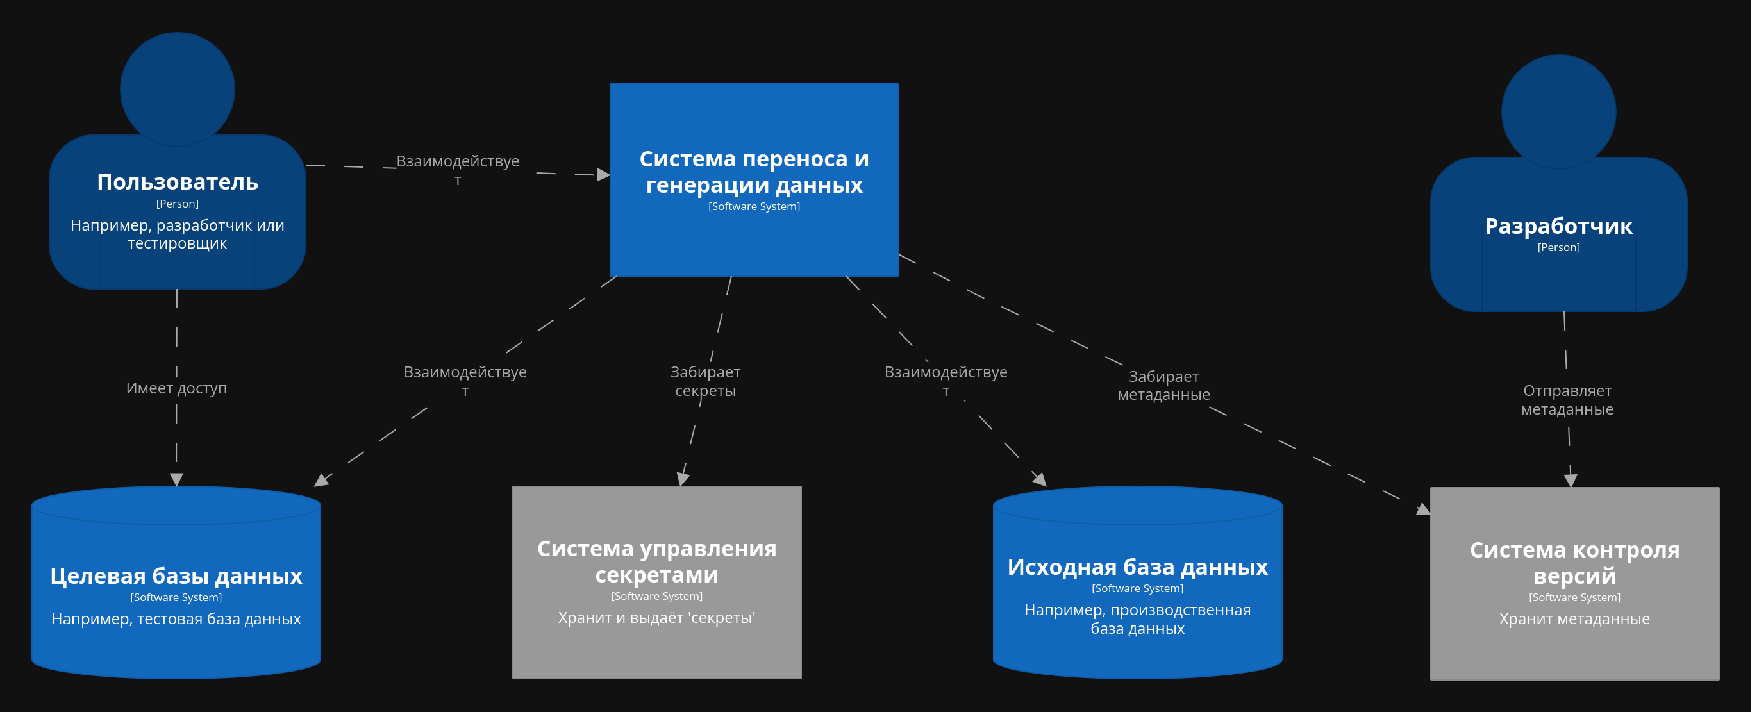
\includegraphics[width = 13cm]{img/structurizr-SystemLandscape-cut}
	\end{center}
\end{frame}

\begin{frame}
\frametitle{Архитектура системы}
	Система переноса и генерации данных

	\begin{center}
		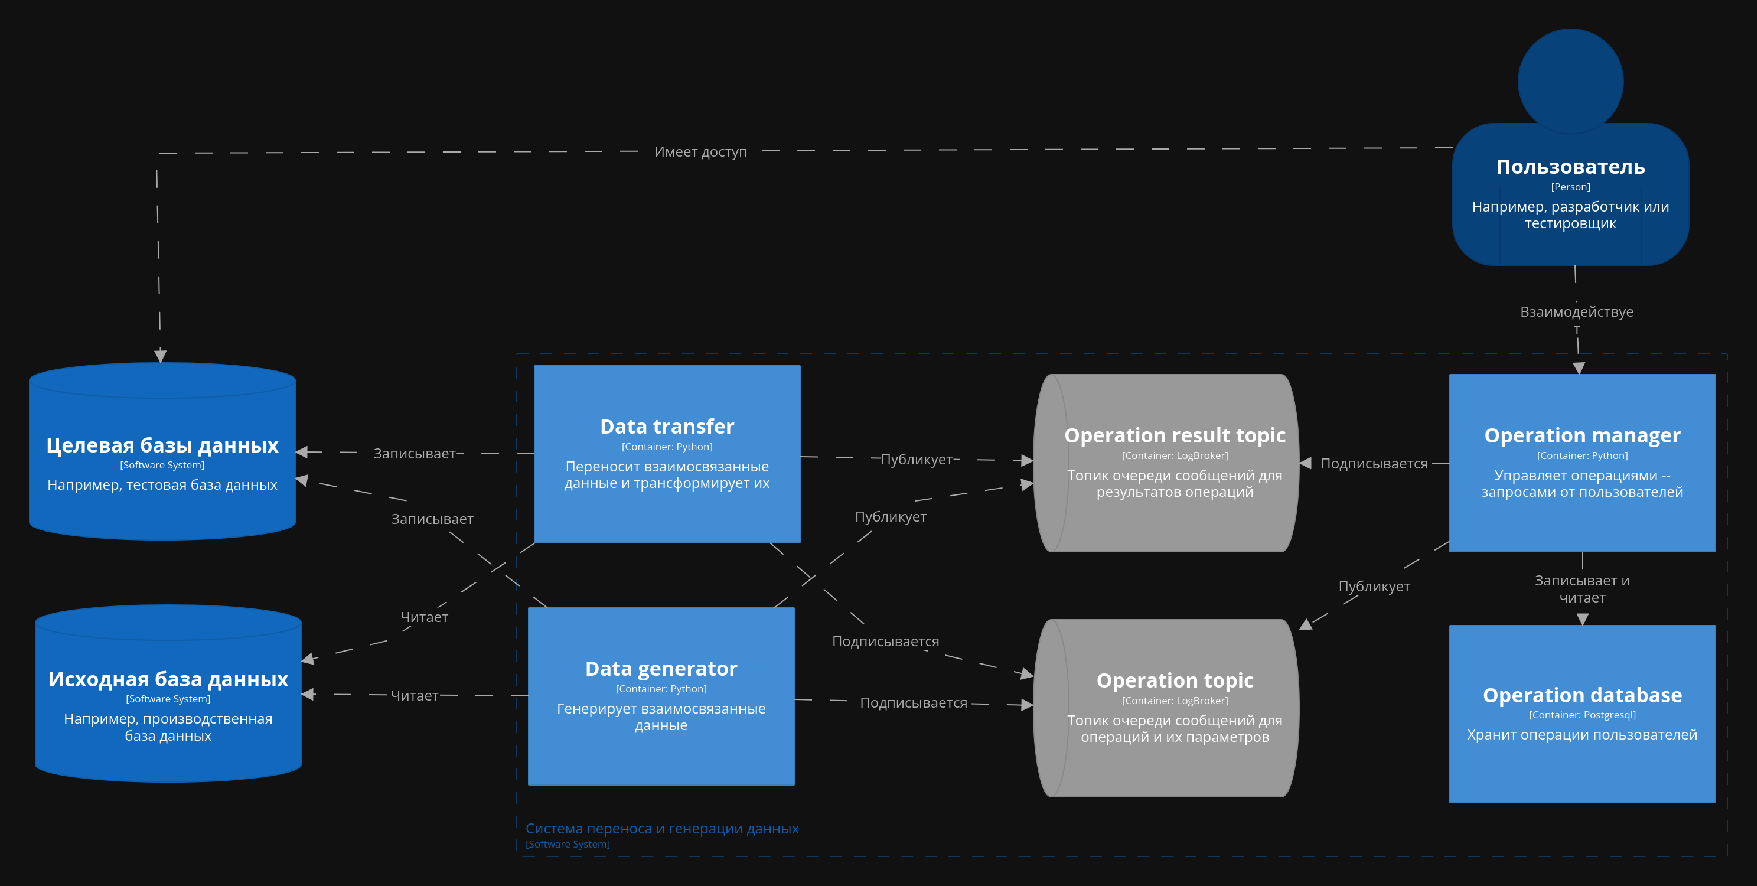
\includegraphics[height = 6cm]{img/structurizr-Containers-cut}
	\end{center}
\end{frame}


\begin{frame}
\frametitle{Архитектура системы}
	Компоненты Data Transfer

	\begin{center}
		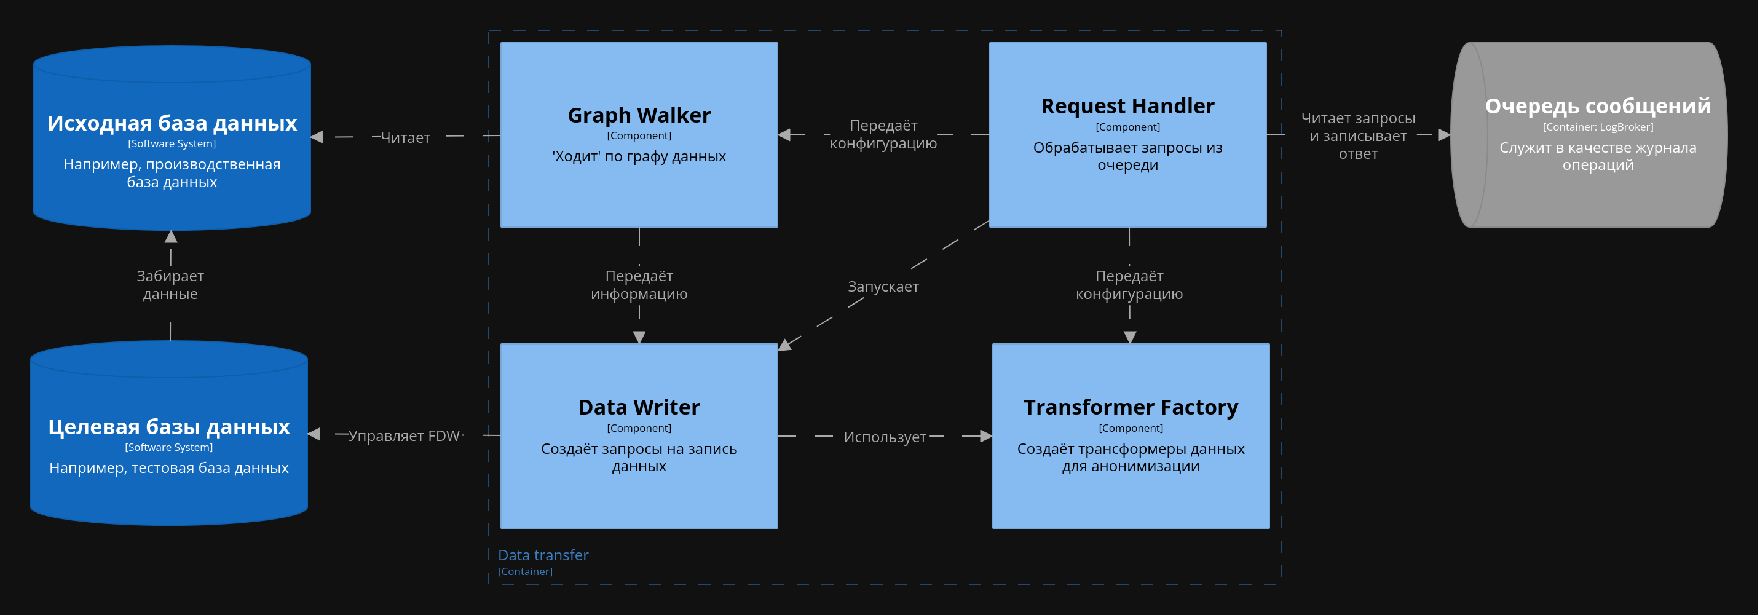
\includegraphics[width = 13cm]{img/structurizr-DataTransferComponents-cut}
	\end{center}
\end{frame}


\begin{frame}
\frametitle{Метаграфы}
	Предпосылки к использованию метаграфов:

	\begin{itemize}
		\item система данных в БД и их взаимосвязей напоминает граф,
		\item классические графы не подходят из-за сложной модели объектов в БД.
	\end{itemize}

	Пусть $MG = \langle V, MV, E, ME \rangle$ -- метаграф, где $V$ -- множество вершин, $MV$ -- множество метавершин, $E$ -- множество рёбер, $ME$ -- множество метарёбер.
\end{frame}


\begin{frame}
\frametitle{Метаграфы}
	Пример базы данных

	\begin{center}
		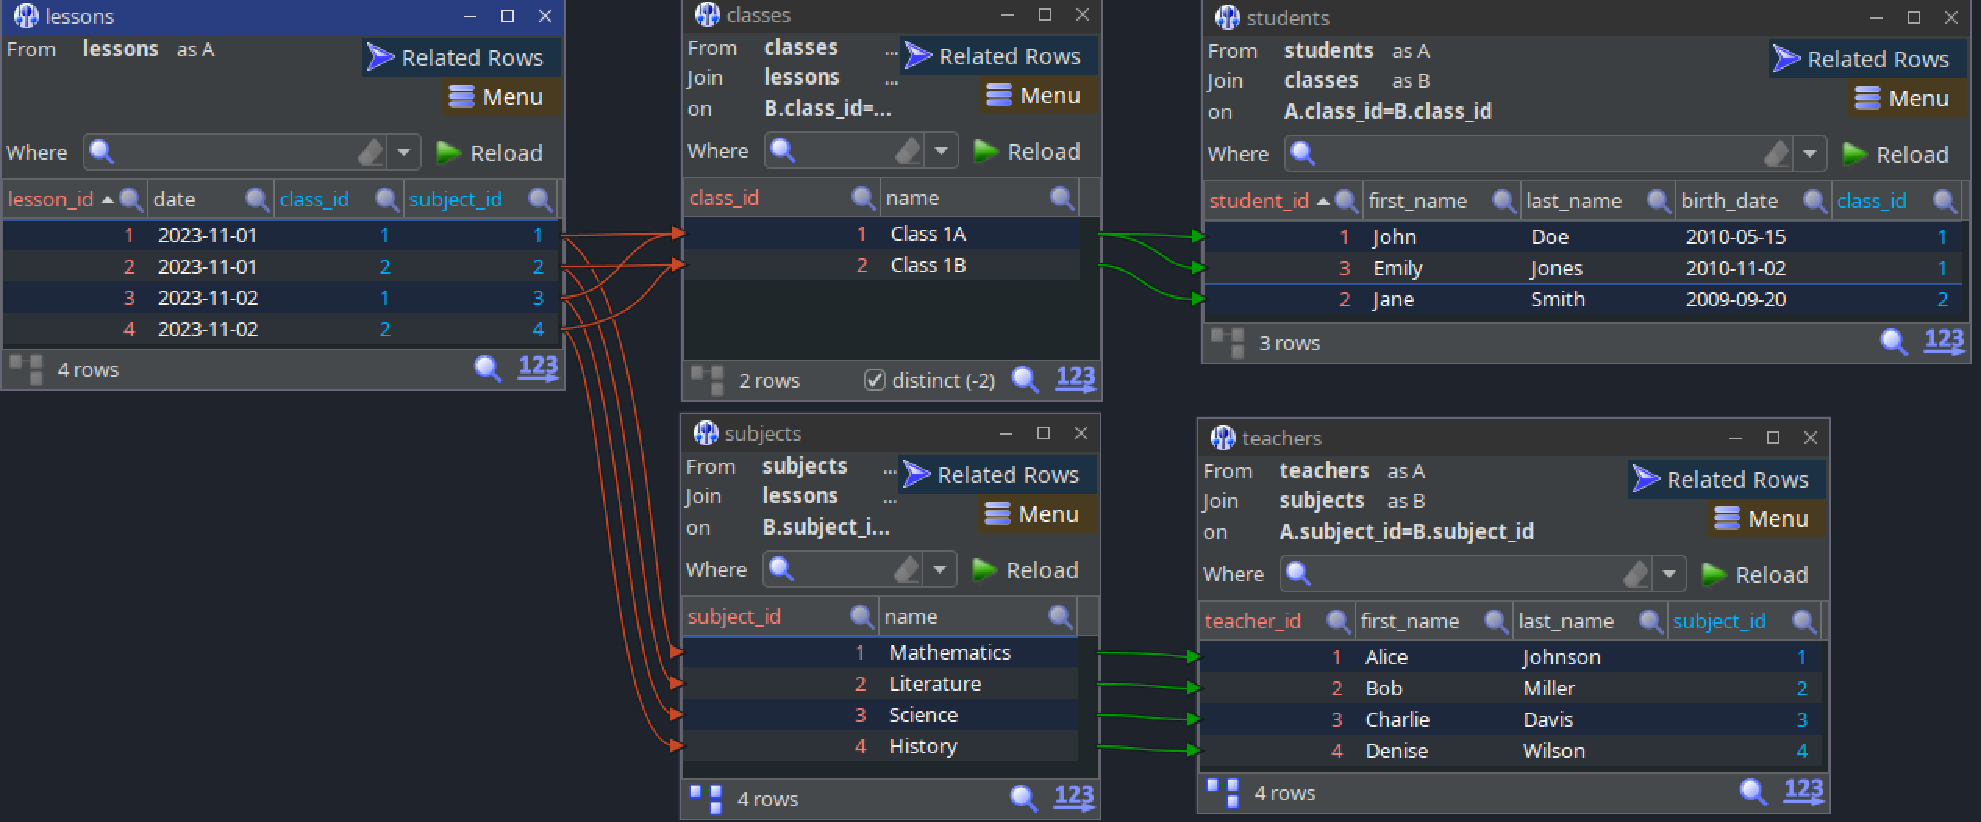
\includegraphics[width = 13cm]{img/jailer-example-db}
	\end{center}
\end{frame}


\begin{frame}
\frametitle{Метаграфы}
	Графическое отображение метаграфа

	\begin{center}
		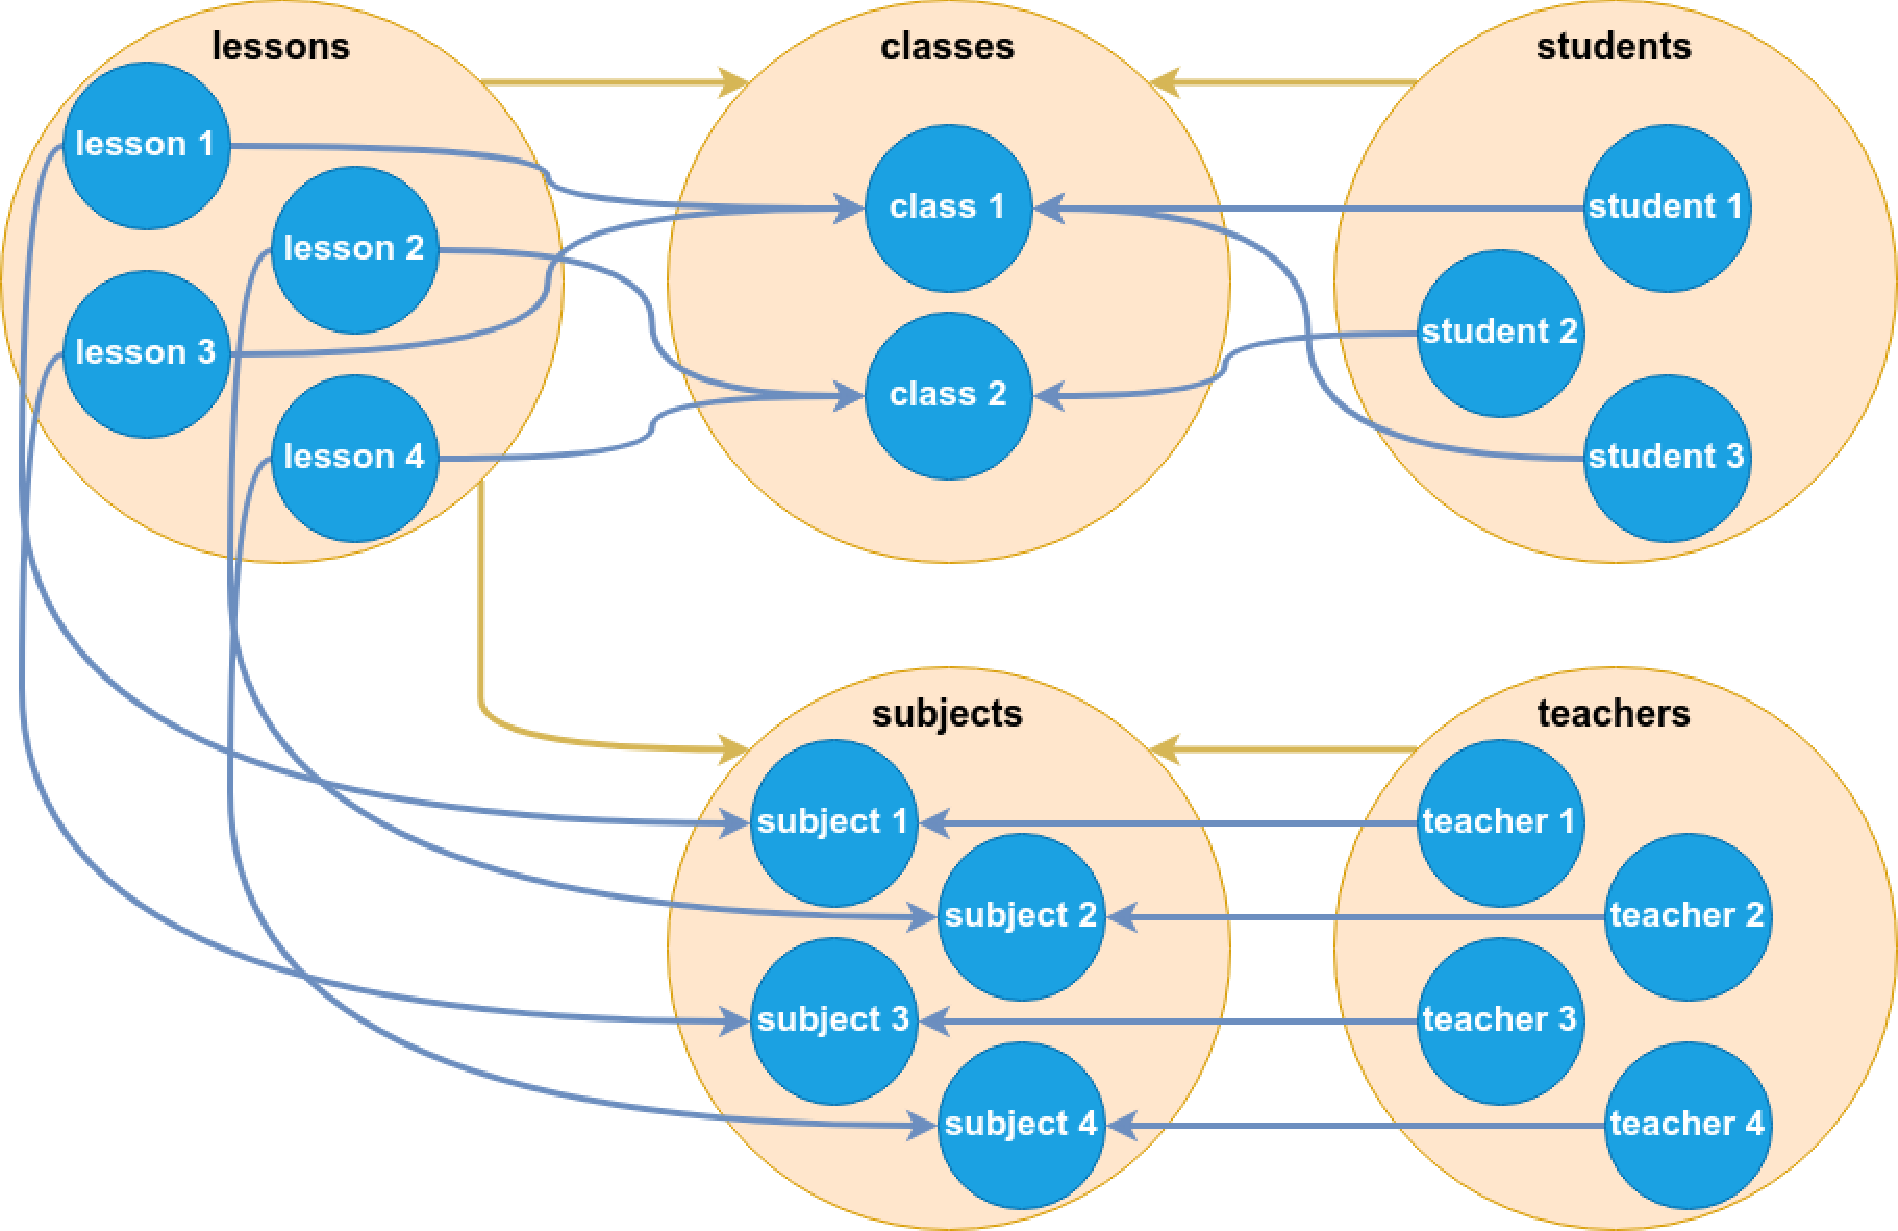
\includegraphics[height = 6cm]{img/drawio-metagraph}
	\end{center}
\end{frame}


\begin{frame}
\frametitle{Алгоритм обхода данных}

	\begin{center}
		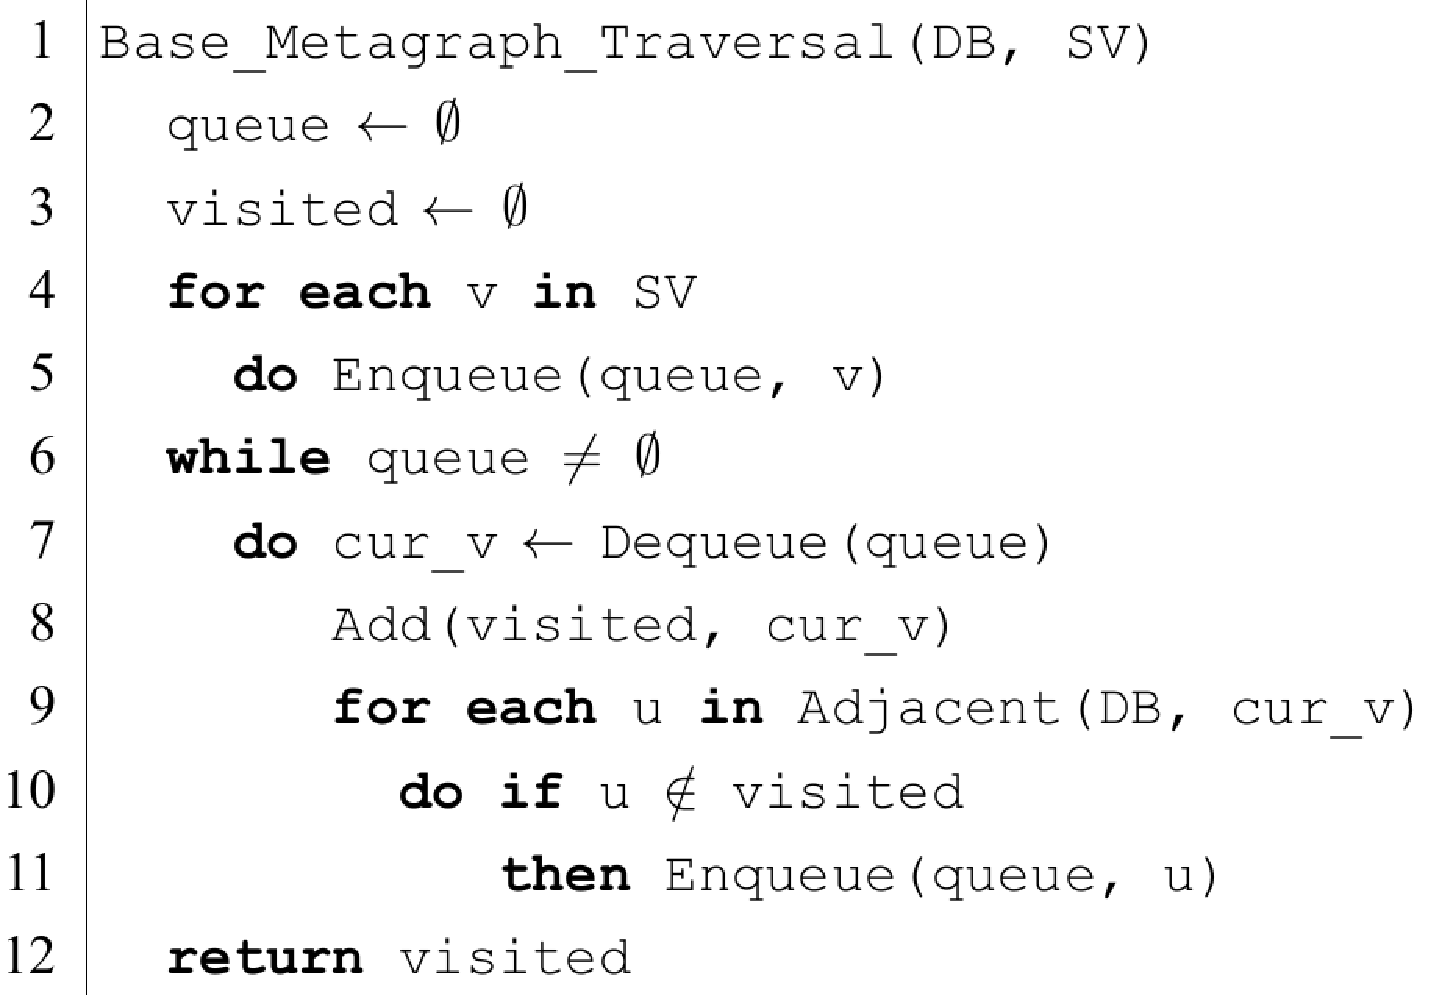
\includegraphics[height = 6.5cm]{img/algorithm-base}
	\end{center}
\end{frame}


\begin{frame}
\frametitle{Алгоритм обхода данных}

	\begin{center}
		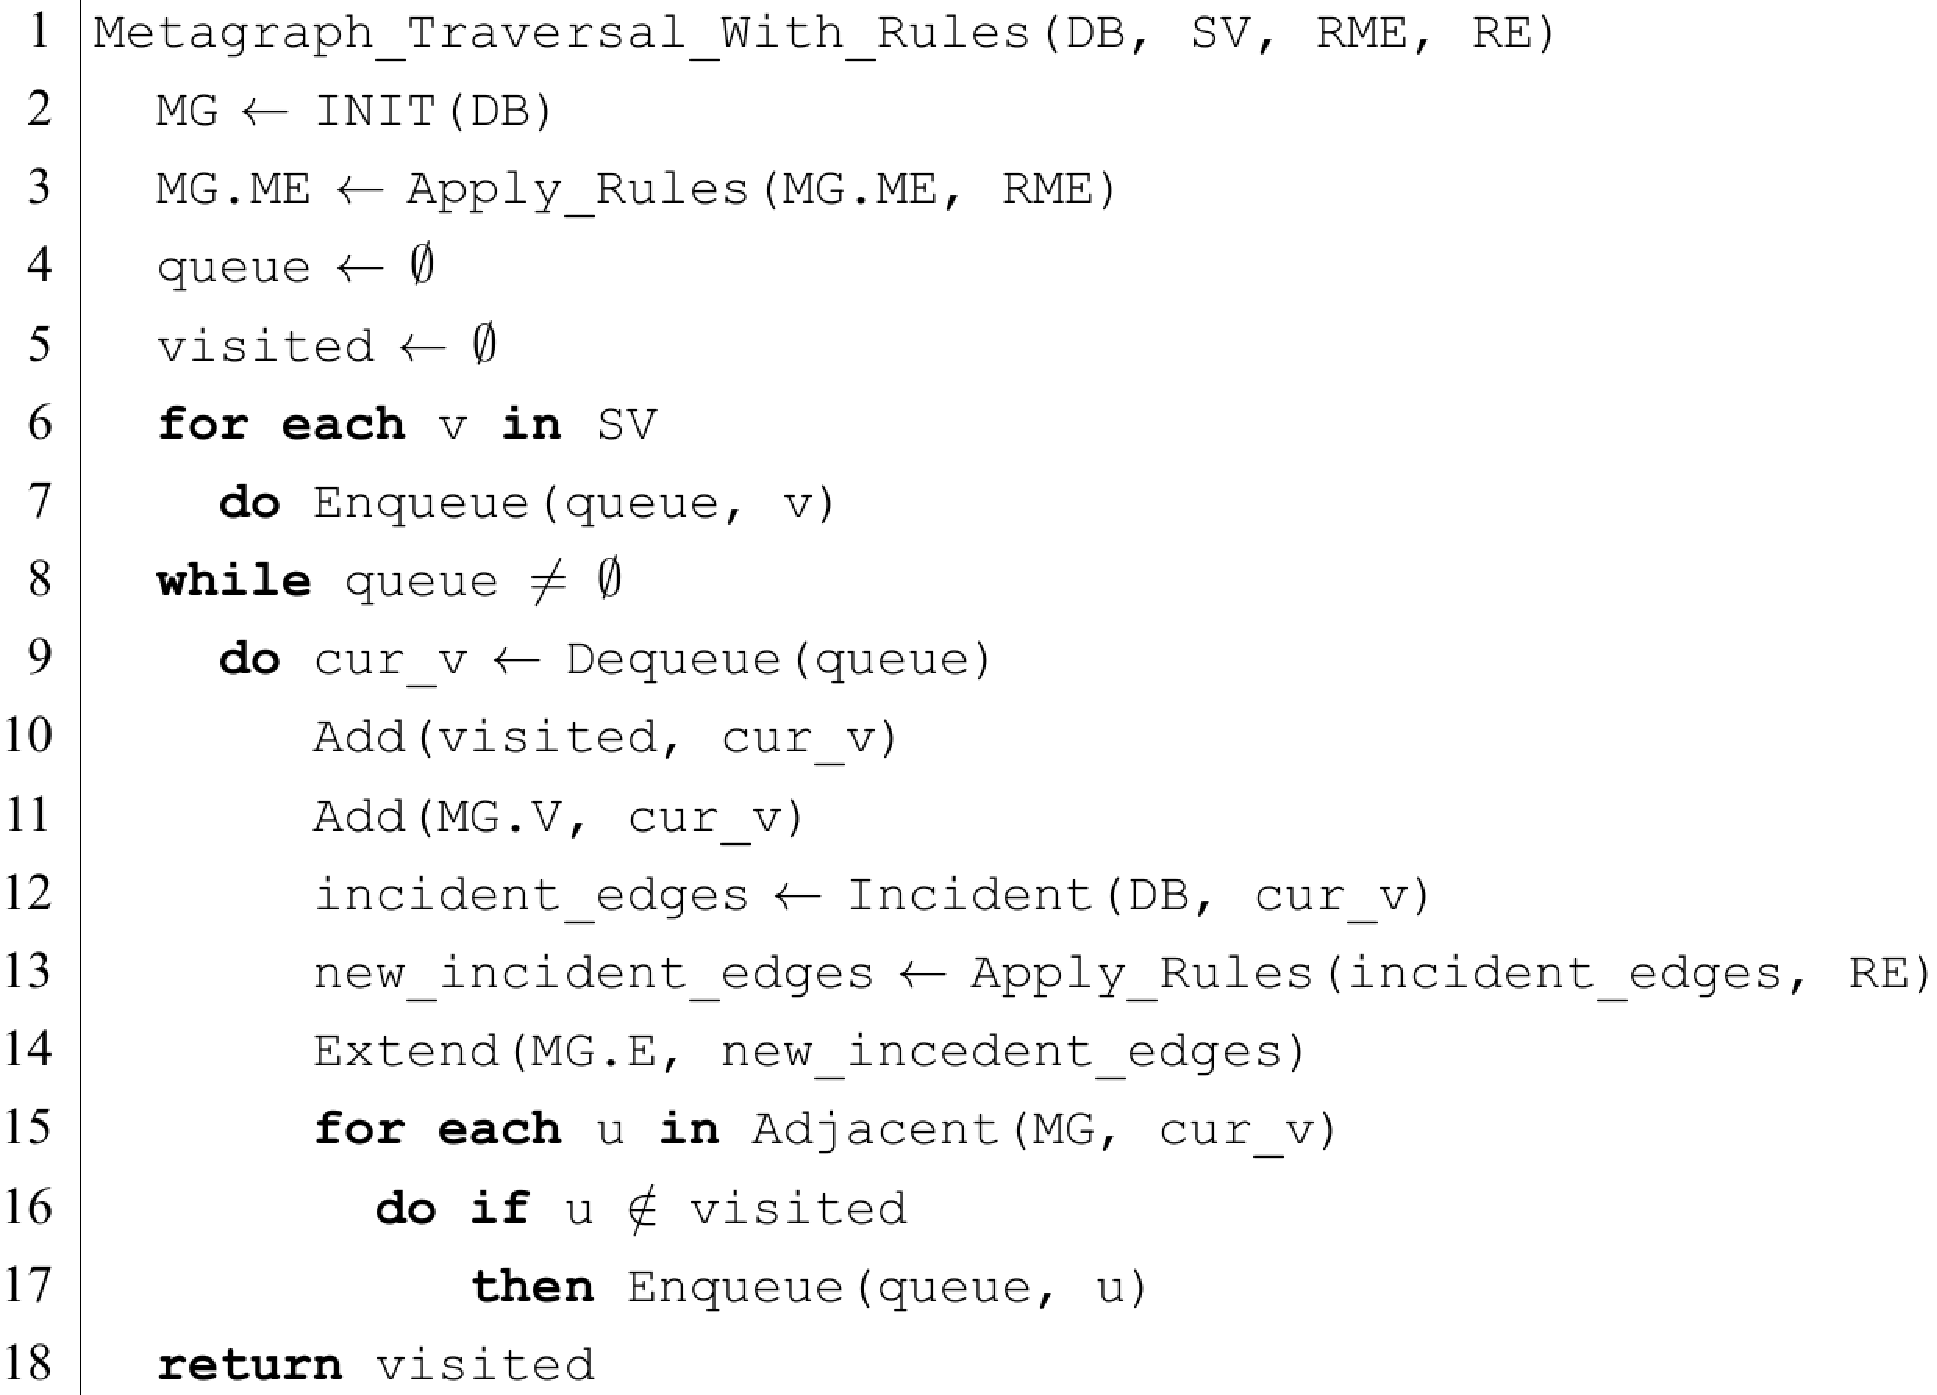
\includegraphics[height = 6.5cm]{img/algorithm-with-rules}
	\end{center}
\end{frame}


\begin{frame}
\frametitle{Язык описания данных}
	Примеры описания метаданных для переноса данных

	\begin{center}
		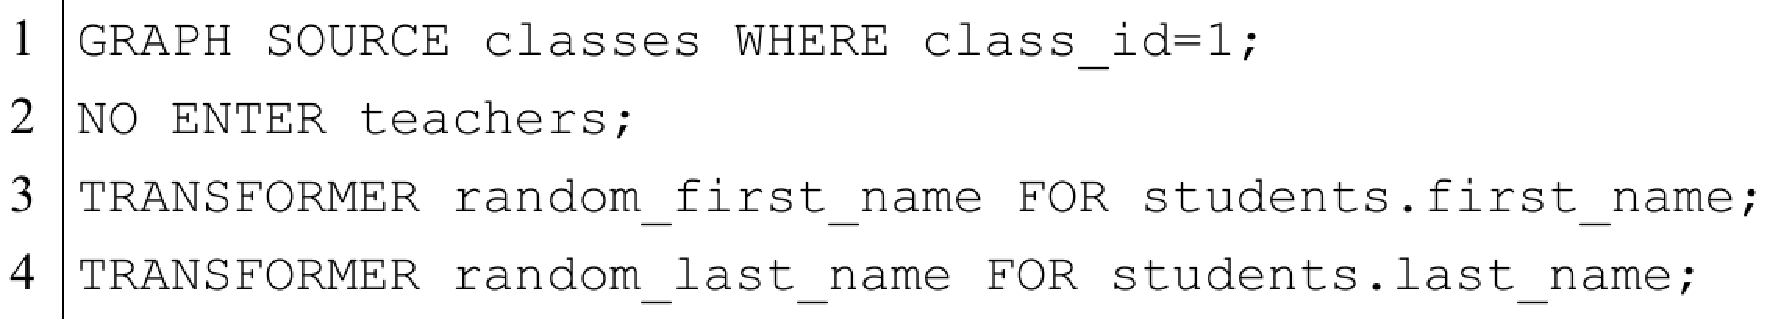
\includegraphics[width = 12cm]{img/language-1}
	\end{center}

	\begin{center}
		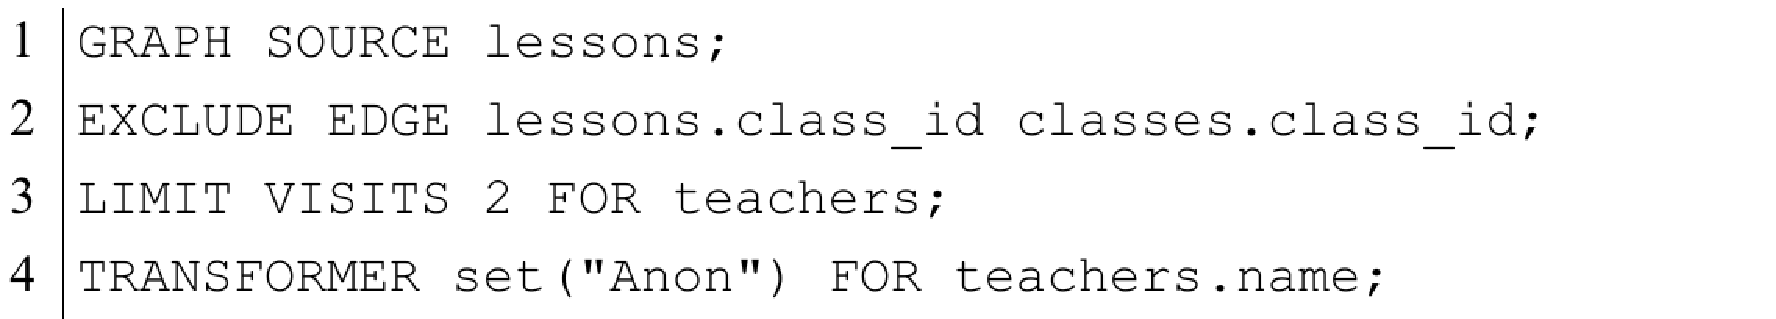
\includegraphics[width = 12cm]{img/language-2}
	\end{center}
\end{frame}


\begin{frame}
\frametitle{Язык описания данных}
	Пример описания метаданных для генерации данных

	\begin{center}
		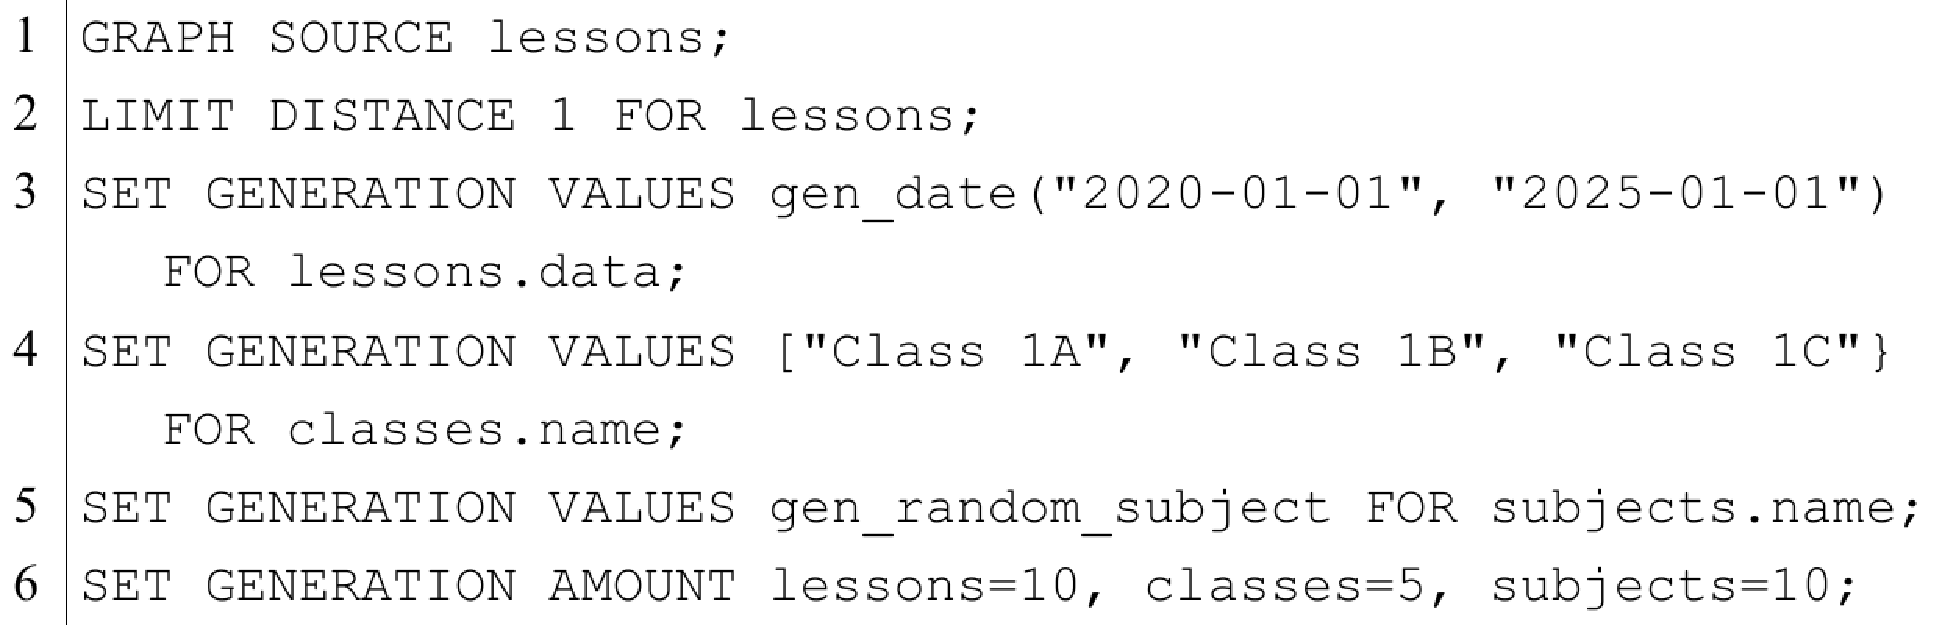
\includegraphics[width = 12cm]{img/language-3}
	\end{center}
\end{frame}


\begin{frame}
\frametitle{Прототип}
	Возможности:

	\begin{itemize}
		\item CLI,
		\item перенос взаимосвязанных данных,
		\item работа со схемами.
	\end{itemize}
\end{frame}


\begin{frame}
\frametitle{Тесты производительности}
	Тестовая база данных: 4.5 ГБ, 44739072 записей.

	\begin{center}
		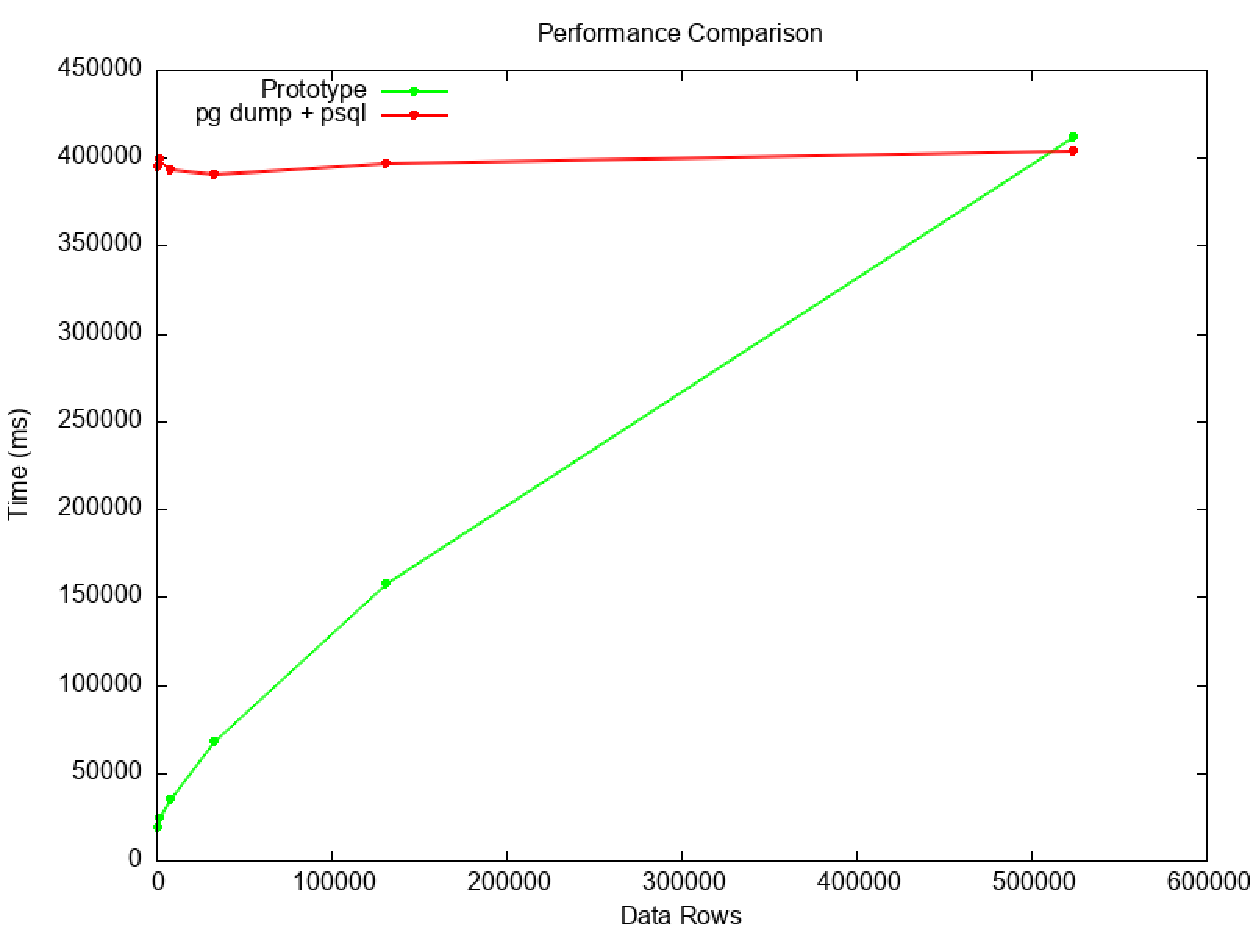
\includegraphics[height = 6cm]{img/benchmark}
	\end{center}
\end{frame}


\begin{frame}
\frametitle{Анализ результатов}
	\textbf{Результаты}:

	\begin{itemize}
		\item спроектирована безопасная и надёжная архитектура,
		\item разработан удобный язык описания метаданных, похожий на привычный SQL,
		\item разработан прототип, который показал высокую скорость работы при переносе небольшого количества взаимосвязанных данных.
	\end{itemize}

	\textbf{Что можно улучшить}:

	\begin{itemize}
		\item производительность,
		\item понимание описания метаданных и алгоритма.
	\end{itemize}

\end{frame}


\begin{frame}
\frametitle{Описание программной разработки}
	Ссылки на код грамматики и код прототипа (скоро будет).

	\begin{center}
		
\includegraphics[height = 6cm]{img/qr-code-relatio-lang}
	\end{center}
\end{frame}

\end{document}
